\documentclass{article}
% --- Packages (formatting only; wording unchanged) ---
\usepackage[margin=1in]{geometry} % 1 inch margins all around
\usepackage{graphicx,xcolor}
\usepackage{booktabs}
\usepackage{amsmath}
\usepackage{float}      % for [H] exact placement
\usepackage{placeins}   % for \FloatBarrier
\usepackage{caption}
\captionsetup{justification=Centering, skip=0.5\baselineskip}
\usepackage{graphicx} % Required for inserting images
\usepackage[numbers, square]{natbib}
\usepackage{enumitem}

\title{\vspace{-2cm}MAT292 Final Project: TITLE}
\author{Group 11: Arthur Chen - Jerry Jiang - Ben Lian}
\date{October 3, 2025}

\begin{document}

\maketitle

\section{Motivation and Objectives (Why \& What?)}
"The Video Game Industry (VGI) is a highly innovative and rapidly growing sector [...] with significant economic and social implications. [Yet] the literature remains fragmented and lacks a coherent framework for understanding its complex nature and underlying dynamics." \cite{GOH2023100100} We find that predicting the population of gamers over time can apply our research on the interplay between technological advances, affordability, accessibility, and market saturation.\\

\noindent Our goal is to develop a differential equation-based prediction model to illustrate how the personal computer (PC) gamer population changes over time due to factors such as commercial hardware improvements, affordability, accessibility, and market saturation. Beyond simple numerical estimations, we aim to explore the involvement of emerging technologies (VR, cloud gaming, or quantum computing) in accelerating growth or leading to new technological trends.

\section{Mathematical and Computational Background (What \& How?)}
Our project uses mathematical concepts from MAT292 to model our analysis of the relationship between PC video game players and tech growth. In our elementary stage, we intend to apply Ordinary Differential Equations (ODE) modeling, focusing on models of logistic growth, bass adoption/diffusion, and compartmental models in epidemiology. Machine learning implementations can focus on adoption dynamics of networks, accounting for the network of social connections. 

\begin{figure} [H]
    \centering
    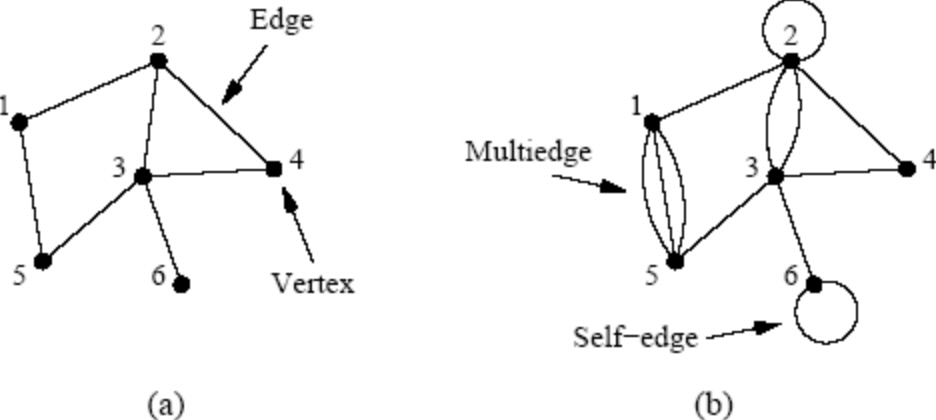
\includegraphics[width=0.5\linewidth]{Image.jpeg}
    \caption{By using networks that place individuals as nodes in a graph and adoption spreading along edges, our model can reflect the practical influences of local relationships \cite{10.1093/acprof:oso/9780199206650.003.0006}.}
    \label{fig:GraphNodeFigure}
\end{figure}

% Mention more about the metrics like in the doc as well as computation


\subsection{Logistic Growth Model}
As mentioned in Lecture 07 (Murdock), the logistic equation with carrying capacity and threshold can be applied: 

\begin{equation}
    \frac{dP}{dt} = rP \left(1 - \frac{P}{T}\right)\left(1 - \frac{P}{K}\right)
\end{equation}

\noindent $P$ is defined as the gamer population, $r$ is the growth rate, $K$ is the carrying capacity of the game servers and $T$ is the population threshold necessary for the game to be financially sustainable for the company.  

\subsection{Bass Adoption/Diffusion Model}
The growth of video games is a form of consumer adoption of technology, which the Bass Model \cite{916272ae-6b7a-3e62-b7e2-5747187dae7b, f1542a98-16de-3de1-ac28-c48c9779e63f}, can inspire our analysis: 

\begin{equation}
    \frac{dN}{dt} = p \left(M - N\right) + q \frac{N}{M} \left(M - N\right)
\end{equation}

\noindent where $M$ is the gamer population the market can adopt, $p$ is the coefficient of "innovation" determined by external influences (e.g., advertising, media, marketing), and $q$ is the coefficient of "imitation", determined by internal influences of word of mouth, peer-to-peer spread. Particularly, the first term of "innovators," $p \left(M - N\right)$, describes those who adopt playing a game due to marketing; while the second term, $ q \frac{N}{M} \left(M - N\right) $, are the "imitators" joining the game under the influence of current players. 

% Can mention parallels such as innovators and imitators, which the gamer 
% population is composed of. Add later if necessary. 

\subsection{Compartmental Epidemics Model}
Compartmental modelling divides the population into multiple groups, focusing on population shifts between different compartments, each with their own growth rates. Based on the Susceptible, Infectious, and Recovered individuals (SIR) model \cite{Hethcote2000Mathematics}, we chose the categories of Potential Gamers, $S$; Active Gamers, $I$, and Retired/Past Gamers, $R$:

\begin{equation}
\frac{dS}{dt} = -\beta S I, 
\qquad \frac{dI}{dt} = \beta S I - \gamma I, 
\qquad \frac{dR}{dt} = \gamma I
\end{equation}

\noindent Said equations are useful in studying churn rates, "the rate at which customers stop doing business with an entity" \cite{INVESTOPEDIA2025CHURN}. This allows investigation of players returning to a game after retirement. 



\section{Timeline (How?)}
Our group plans to achieve the following weekly milestones starting \textbf{Sunday, October 5}: \\

\begin{enumerate}[nosep]
    \item \textbf{Week of Oct. 5}: Review literature on adoption models, finalize metrics, gather data sources.
    \item \textbf{Week of Oct. 12}: Define base ODE framework.
    \item \textbf{Week of Oct. 19}: Extend the model to incorporate factors of hardware growth, affordability, accessibility and market saturation.
    \item \textbf{Week of Oct. 26}: Implement computational simulations in Python. 
    \item \textbf{Week of Nov. 2}: Analyze baseline predictions and scenario testing (e.g., with/without quantum computing).
    \item \textbf{Week of Nov. 9}: Organize results, integrate graphs/visuals, refine equations.
    \item \textbf{Week of Nov. 16}: Finalize report, verify reproducibility of code, and review for submission.
    \item \textbf{Week of Nov. 23}: Extra time reserved as safety for any unforeseen circumstances.

\end{enumerate}


\section{Expected Outcomes}
Our group plans to deliver the following: 
\begin{itemize} [nosep]
    \item \textbf{A predictive ODE-based model estimating the global gamer population over time}.
    \item \textbf{Integration of at least 3 distinct modelling techniques}: logistic growth, Bass diffusion, SIR models, etc. 
    \item \textbf{Case Study}: compare predicted results with hypothetical technological shocks (e.g., sudden VR breakthroughs lowering costs and increasing adoption).
    \item \textbf{Verification and Validation}: present graphs, simulations and sensitivity analyses to interpret the effect of each factor.
    \item \textbf{Discussion}: explore limitations of the model and future enhancements through refined data and/or nonlinear systems.

\end{itemize}


\bibliographystyle{plain} % Or abbrv, unsrt, etc.
\bibliography{ref}
\end{document}